\chapter{Data structure}\label{ch:structure}

The data studied in this work can be represented as component systems. These component systems can be represented by a two dimensional matrix in which rows represent components and columns are the possible realizations buildable given subset of the components. The entries of this matrix are the number of the components on the row needed during the realization of the column. In figure~\ref{fig:componetstable} an example of this kind of matrices.

%%data definitions
\section{Component systems}
\begin{figure}[htb!]
\centering
\begin{tabular}{cc}
&Realizations\\
 \rotatebox[origin=c]{90}{Components}&
  $\left(\begin{array}{ccccc}{n_{11}} & {n_{12}} & {n_{13}} & {\dots} & {n_{1 R}} \\ {n_{2 1}} & {n_{2 2}} & {n_{2 3}} & {\dots} & {n_{2 R}} \\ {\vdots} & {\vdots} & {\vdots} & {\ddots} & {\vdots} \\ {n_{N 1}} & {n_{N 2}} & {n_{N 3}} & {\dots} & {n_{N R}}\end{array}\right)$\\
\end{tabular}
\caption{Structure of a matrix representing component systems with $i=0\dots N$ rows and $j=0\dots R$ columns.}
\label{fig:componetstable}
\end{figure}
The most common example of such systems is a set of books, in this case one puts on the rows the words in the whole vocabulary and the books' titles on the columns; the entry that corresponds to row $i$ and column $j$ is the number of times the word $i$ appears in book $j$. The same happens if one considers Wikipedia's pages. Other examples are Lego$\textsuperscript{\tiny\textregistered}$ sets where components are the Lego$\textsuperscript{\tiny\textregistered}$ bricks and realizations Lego$\textsuperscript{\tiny\textregistered}$ packages and protein domains; all these were described and well studied in~\cite{mazzolini2018heaps, Mazzolini2018zipf}.

Given a matrix with $N$ components on the rows and $R$ realizations on the columns and relative abundances $n_{ij}$ as the entries, it is interesting to study some quantities that are universal and general characteristics of component systems.

First of all, the \textbf{occurrence} of a component is defined as 
\begin{equation}\label{eq:occurrence}
O_i=\frac{\sum_{j=1}^{R}(1-\delta_{n_{ij},0})}{R}
\end{equation}
and is the fraction of realizations in which the component's abundance is not null. A component that is present in all the realizations has got $O_i=1$, the ensemble of all components with $O_i=1$ is known as the \textbf{core}. Components with high ($\simeq 1$) occurrence are present in mostly all realizations of the datasets, in linguistics articles (such as \textit{the}) are present everywhere, so they have high occurrence. Components with low occurrence $\simeq 0$ are present only in a few realizations and are the most specific ones~\cite{altmann2016statistical}.

The sum across all columns is called \textbf{abundance} of a component and is defined as:
\begin{equation}\label{eq:abundance}
a_i=\sum_{j=1}^{R}n_{ij};
\end{equation}
dividing this by the global abundance 
\begin{equation}
  a=\sum_{i=1}^{N}a_i
\end{equation}
naturally brings to the \textbf{frequency of a component} in the whole corpus
\begin{equation}\label{eq:fi}
f_i=\frac{a_i}{\sum_{c=1}^{N}a_{c}}.
\end{equation}
Dividing the abundance of a component by the sum of all abundances in a realization gives the \textbf{frequency} of the component in that specific realization
\begin{equation}
f_{ij}=\frac{n_{ij}}{\sum_{c=1}^{N}n_{cj}}.
\end{equation}

The sum of all abundances in the same realization
\begin{equation}\label{eq:size}
M_j=\sum_{c=1}^{N}n_{cj}
\end{equation}
represent the \textbf{size} of the realization.

It is expected that frequencies distribute according to the so-called Zipf's law
\begin{equation}\label{eq:zipf}
f_i\propto r_i^{-\alpha}
\end{equation}
where $r$ is the rank: the position of a component when sorting all components by their frequencies in the whole dataset.

%%universal laws
\section{Universal laws in RNA-Seq}\label{sec:universallaws}
\subsection{TCGA}
Analysing TCGA dataset~\cite{grossman2016toward} the first interesting analysis is to plot the sorted abundance, this gives the so called Zipf's law. The analysis were made considering \textit{Gene Expression Quantification} as data type, \textit{Transcriptome Profiling} as data, \textit{RNA-Seq} as experimental strategy, \textit{HTSeq - Counts} or \textit{HTSeq - FPKM} as workflow type. $5000$ samples were downloaded and analysed.
\begin{figure}[htb!]
    \centering
    \begin{minipage}{0.45\textwidth}
    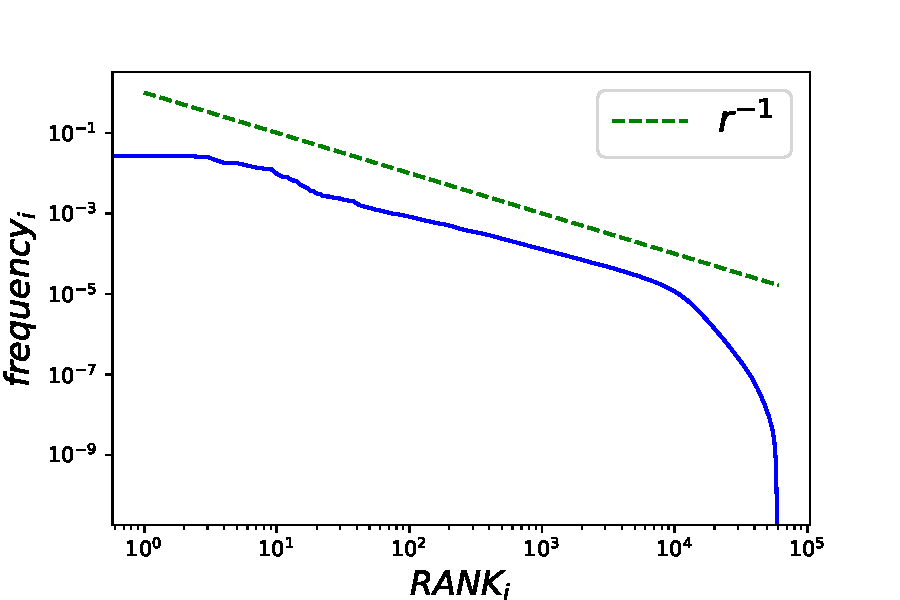
\includegraphics[width=0.95\linewidth]{pictures/structure/tcga/globalzipf_fpkmall.pdf}
    \end{minipage}
\hspace{3mm}
    \begin{minipage}{0.45\textwidth}
    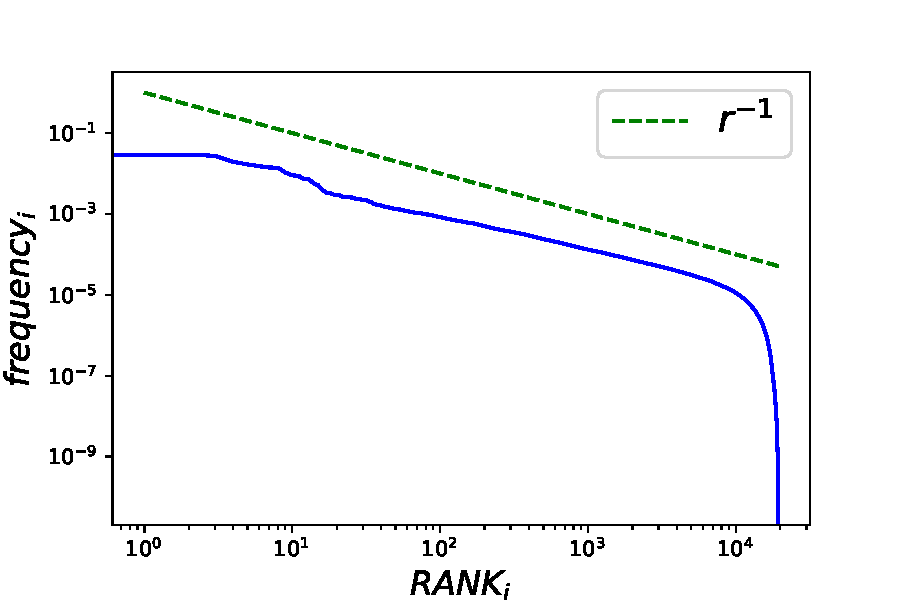
\includegraphics[width=0.95\linewidth]{pictures/structure/tcga/globalzipf_fpkm.pdf}
    \end{minipage}
    \caption{Zipf's law from FPKM normalised data. On the right considering only protein coding genes}
    \label{fig:structure/tcga/globalZipf}
\end{figure}
In figure~\ref{fig:structure/tcga/globalZipf} it is shown the frequency ranked plot. It is interesting that this kind of data distribute according a power law with exponent close to $1$, this same behaviour can be found in completely different systems such as linguistics' ones~\cite{altmann2016statistical}. Another interesting fact is that considering in the analysis also non-coding genes gives a double-scaled power law. This is due to the fact that non coding genes are also more specific and rare, so their frequencies are quite small compared to protein coding genes.

Changing normalisation and considering counts instead of FPKM, the result is quite similar. The power law is more flat, meaning that genes have more similar abundances in the whole dataset. 
\begin{figure}
    \centering
    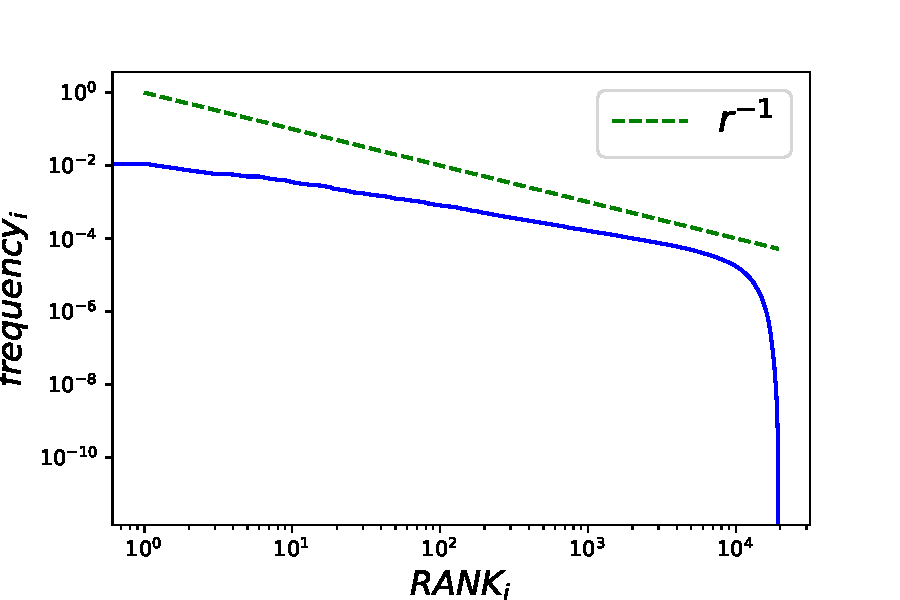
\includegraphics[width=0.8\linewidth]{pictures/structure/tcga/globalzipf_counts.pdf}
    \caption{Zipf's law of protein coding genes considering counts}
    \label{fig:structure/tcga/globalzipf_count}
\end{figure}

\subsection{GTEx}
A pretty similar analysis can be made on GTEx's~\cite{carithers2015novel} healthy samples. RNA sequencing raw counts data were download from file version \textit{2016-01-15 v7 RNASeQCv1.1.8}. All $\sim 11000$ samples available were considered at this time.

\begin{figure}[htb!]
    \centering
    \begin{minipage}{0.45\textwidth}
    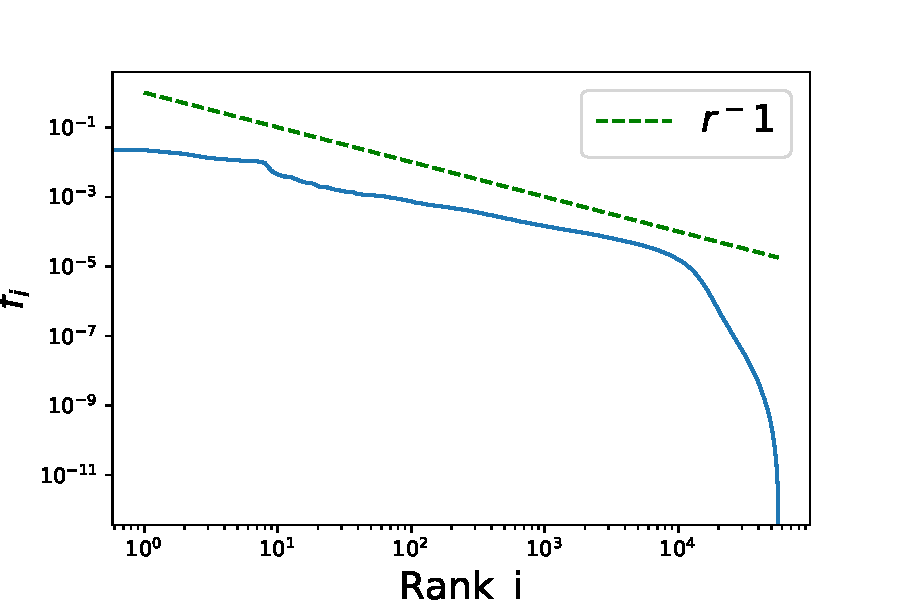
\includegraphics[width=0.95\linewidth]{pictures/structure/gtex/globalZipf.pdf}
    \end{minipage}
    \hspace{3mm}
    \begin{minipage}{0.45\textwidth}
    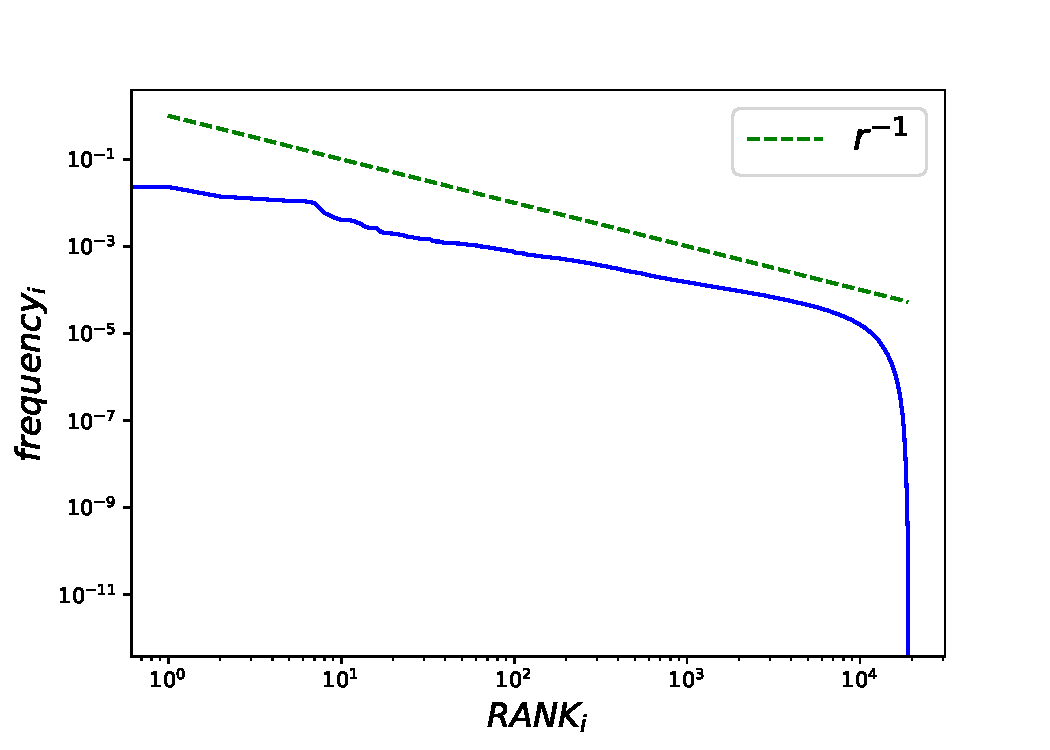
\includegraphics[width=0.95\linewidth]{pictures/structure/gtex/globalZipf_c.pdf}
    \end{minipage}
    \caption{Zipf's law from GTEx count data. On the left all genes considered, on the right only protein coding ones}
    \label{fig:my_label}
\end{figure}
Not surprisingly in the GTEx dataset it is retrieved the same behaviour at this time. The power law with exponent $\simeq 1$ is found and considering non coding genes lead to a knee in the power law.

Going further in the analysis it is possible make an histogram of occurrences defined by~\ref{eq:occurrence}, also known as $U$s.
\begin{figure}[htb!]
    \centering
    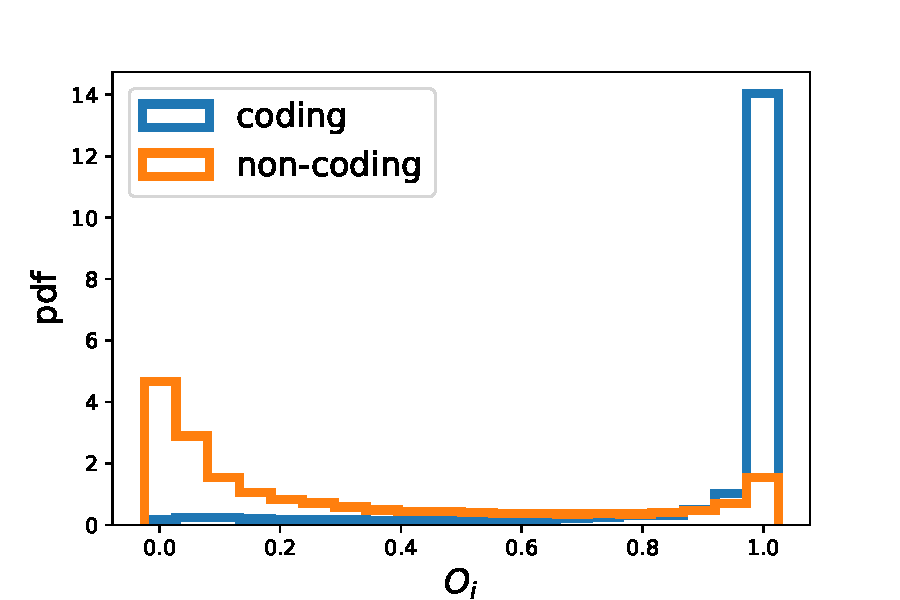
\includegraphics[width=0.9\linewidth]{pictures/structure/gtex/U_gtex_cnc.pdf}
    \caption{The histogram of the occurrences $O_i$}
    \label{fig:structure/gtex/U_cnc}
\end{figure}

Also in this kind of analysis it is possible to see the different behaviour of coding and not coding genes. The protein coding genes express almost in every sample, so their occurrence is near to $1$, non coding genes are more specific, so they are present only in a subset of the dataset and many of the have small occurrence.
\begin{figure}[htb!]
    \centering
    \begin{minipage}{0.45\textwidth}
    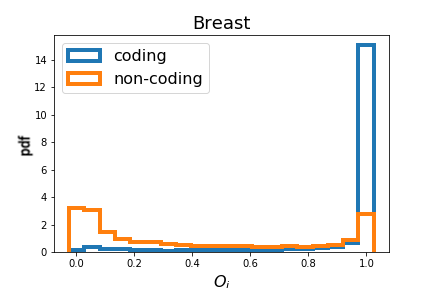
\includegraphics[width=0.95\linewidth]{pictures/structure/gtex/U_Breast.png}
    \end{minipage}
    \hspace{2mm}
    \begin{minipage}{0.45\textwidth}
    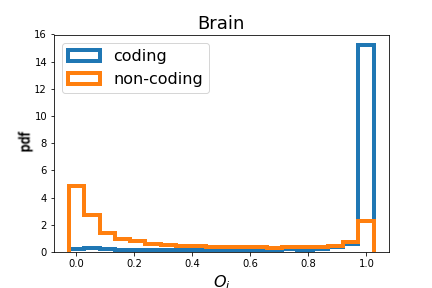
\includegraphics[width=0.95\linewidth]{pictures/structure/gtex/U_Brain.png}
    \end{minipage}
    \caption{Same behaviour is observed looking at one tissue a time.}
    \label{fig:structure/gtex/U_tissues}
\end{figure}
The same behaviour can be observed considering just all samples of a given tissue. In this case $O_i=0$ means that the genes has a non zero expression in just one of the samples of the tissue considered; in other words if a gene never express in a tissue it is not considered when constructing these tissue specific $U$ distributions.

From now on except were explicitly declared analysis will be made considering protein coding genes and counts with no normalisation.


%%null model
\section{Null model construction}\label{sec:nullmodel}
The kind of data considered in this work comes from RNA Sequencing experiments. These experiments use wet biology methods to extract information from samples. If one imagines it exists an unknown function that describes the gene expression across the samples considered, what experimental people do is to sample this function, picking up some genes.

In this section it is described a null model of sampling, this is useful to verify if the data distributions seen are just an effect of this experimental sample or if they carry some useful and interesting information.

As described in~\cite{Mazzolini2018}, a random matrix has to be created. This matrix is a collection of components and realizations exactly as~\ref{fig:componetstable}. The values of each component abundances in each realization $n_{i j}$ are randomly assigned with a probability determined by 
the global abundance in the whole dataset~\ref{eq:abundance}. Values of each column are extracted until the size~\ref{eq:size} is 
reached. Strictly speaking it is a multinomial process with probability
\begin{equation}
P\left( \{ n_i\} ;M\right) =\frac{M!}{\prod_{i=1}^{N} n_i}\prod_{i=1}^N f_i^{n_i}
\end{equation}
where $n_i$ is the number of times the component with frequency $f_i$ appears, being $f_i=\frac{a_i}{\sum_{c=1}^{N}a_{c}}$ as defined in~\ref{eq:fi}.

Figure~\ref{fig:structure/randomsampling} shows an example of this, $M$ components are picked up concerning their frequency in the dataset. The most abundant components, which are also the ones with the highest frequencies (frequency is nothing but the normalized abundance), have a greater probability to be picked up.
\begin{figure}[htb!]
    \centering
    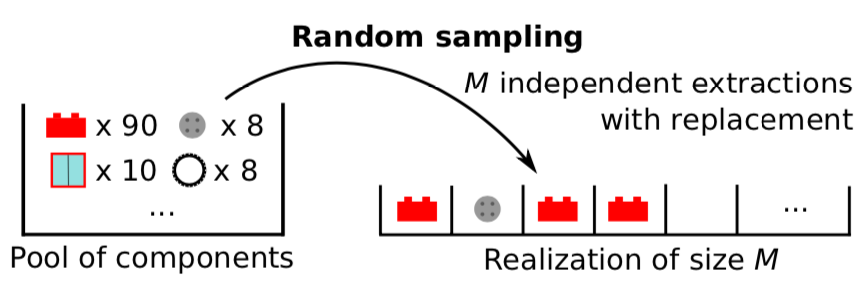
\includegraphics[width=0.8\linewidth]{pictures/structure/randomsampling.png}
    \caption{Random sampling of components to build a realization of size $M$.}
    \label{fig:structure/randomsampling}
\end{figure}

Using this construction on real counts data, by definition the Zipf's law sampled is identical to the data's one.
\begin{figure}[htb!]
\begin{minipage}{0.5\textwidth}
    \centering
    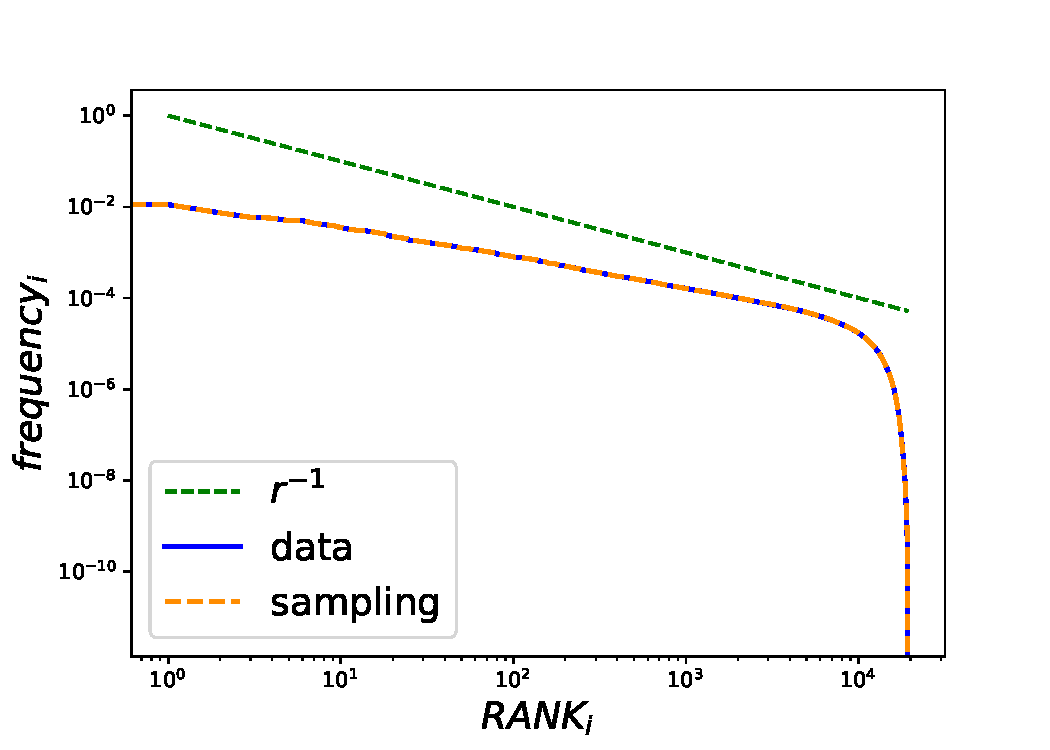
\includegraphics[width=0.95\linewidth]{pictures/structure/tcga/globalzipf_null.pdf}
\end{minipage}
\hspace{2mm}
\begin{minipage}{0.5\textwidth}
    \centering
    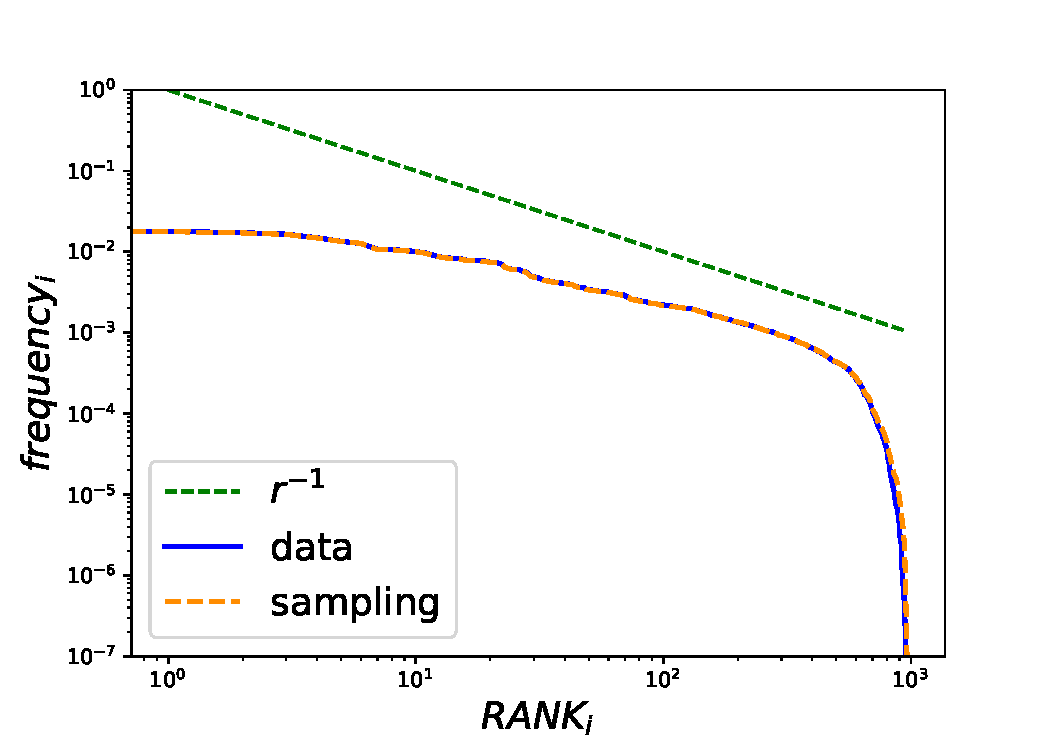
\includegraphics[width=0.95\linewidth]{pictures/structure/gtex/globalzipf_null.pdf}
\end{minipage}
\caption{Zipf's law sampled; TCGA(left) and GTEx (right). By definition original frequencies and sampled ones are identical.}
\label{fig:structure/globalzipf_null}
\end{figure}
By construction, the distribution of the sizes of the sampling and the data are also identical.
\begin{figure}[htb!]
\begin{minipage}{0.5\textwidth}
    \centering
    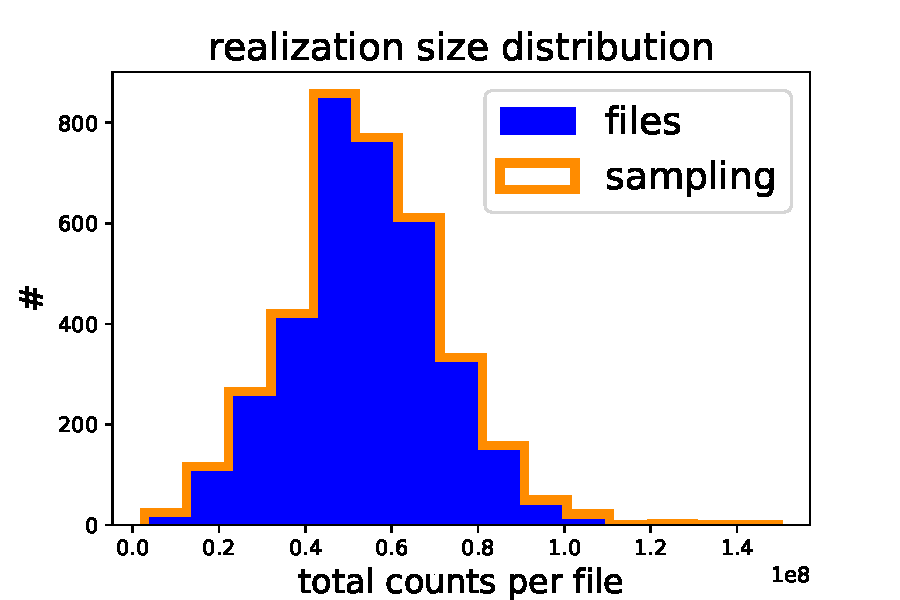
\includegraphics[width=0.95\linewidth]{pictures/structure/tcga/sizeDistr_null.pdf}
\end{minipage}
\hspace{2mm}
\begin{minipage}{0.5\textwidth}
    \centering
    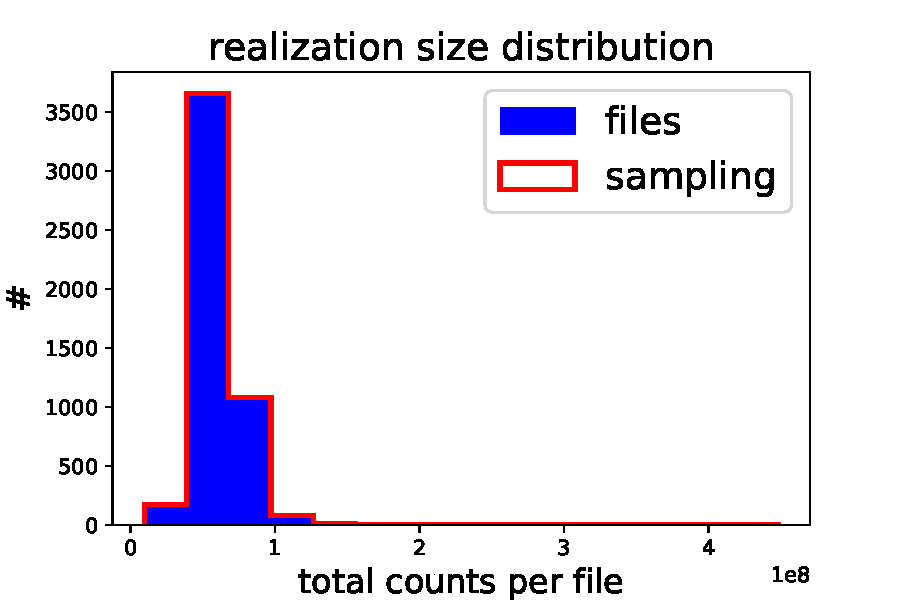
\includegraphics[width=0.95\linewidth]{pictures/structure/gtex/sizeDistr_null.pdf}
    \end{minipage}
\caption{Distribution of sizes $M$; TCGA(left) and GTEx (right). By definition sampling and original sizes are identical.}
    \label{fig:structure/sizeDistr_null}
\end{figure}

Looking at the $U$s in figure~\ref{fig:structure/globalU_null}, it is evident that data behave differently from sampling. This is a signal that the null model is not enough to explain the data matrices. In particular, it is evident that the null model generates the matrices in a manner such that more components have high occurrence comparing to the original data. This can be easily explained, in fact in the real world some genes are highly expressed but only in a subset of the whole dataset; these genes are specific for certain type of samples. The null model gets the information that such genes are highly expressed (they have a high abundance) and so samples these quite often (components with high abundance have a greater chance to be picked up by the null model sampling). This set of genes with $O_i=1$ is called \textbf{core}, in figure~\ref{fig:structure/globalU_null} it is evident the difference between the real one and the sampled one.
\begin{figure}[htb!]
\begin{minipage}{0.5\textwidth}
    \centering
    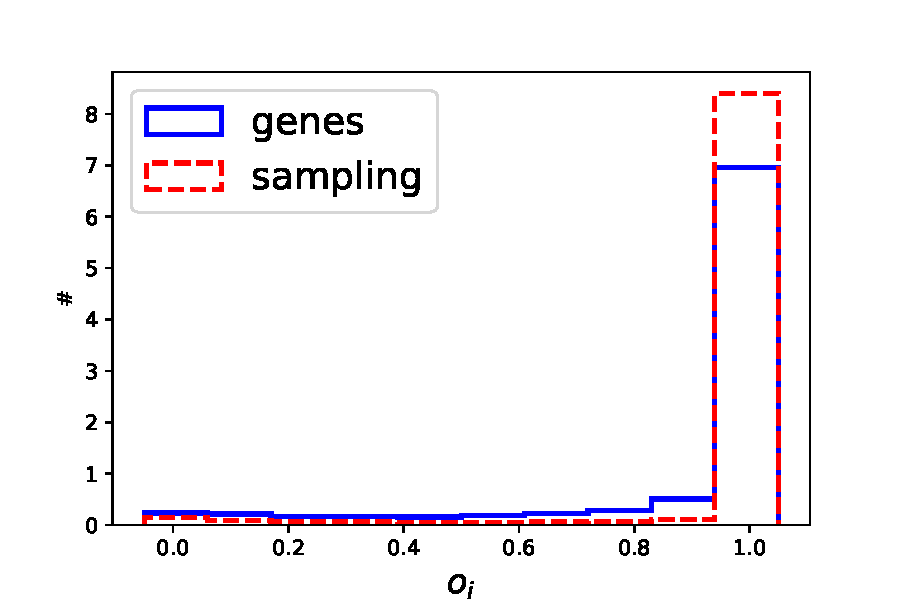
\includegraphics[width=0.95\linewidth]{pictures/structure/tcga/globalU_null.pdf}
\end{minipage}
\hspace{2mm}
\begin{minipage}{0.5\textwidth}
    \centering
    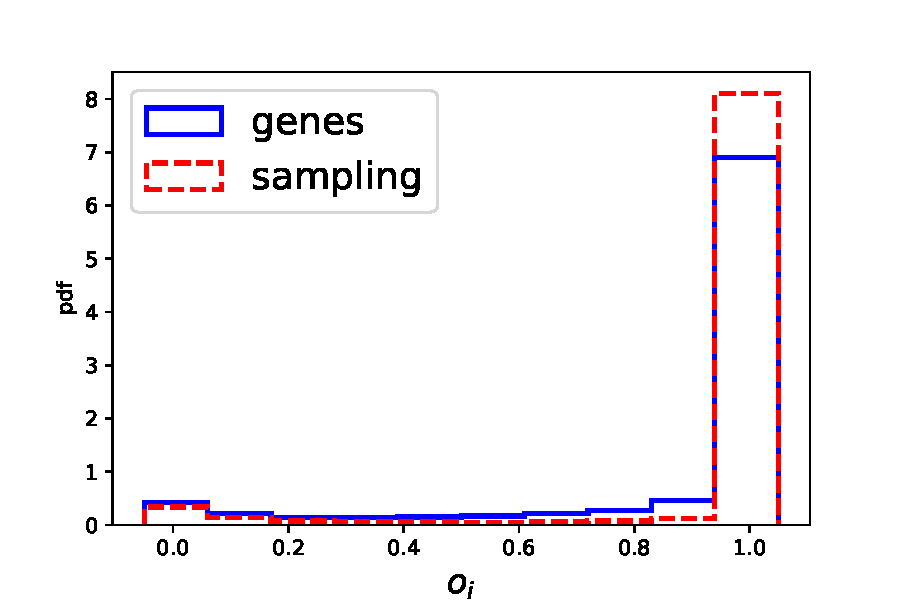
\includegraphics[width=0.95\linewidth]{pictures/structure/gtex/globalU_null.pdf}
    \end{minipage}
\caption{Occurrence distributions; TCGA(left) and GTEx (right). Sampling is reported for comparison.}
\label{fig:structure/globalU_null}
\end{figure}

Plotting on the abscissa the size of samples and on the ordinate the number of genes expressed one point per sample, it is possible to obtain the so-called Heaps's law~\cite{Heaps:1978:IRC:539986}. In figure~\ref{fig:structure/heaps_null} the Heaps' law is presented compared to the one obtained by sampling. Again the curves differ and the null model is not enough to explain the trend. Note that each data point shares the abscissa with a sampling one (figures~\ref{fig:structure/sizeDistr_null} are nothing but the histograms of the abscissas of~\ref{fig:structure/heaps_null}). Moreover, it is interesting that the ordinate does not start from zero, this happens because there are a lot of genes that express everywhere, the core. It happens that the sampling curve is translated above the data's one. This means that to build a sample of size $M$ just by sampling it is necessary to use a greater number of different genes than the number of different genes actually expressed in nature. In other words in the real world only the genes that are really useful in a sample are expressed, and this is not describable just by sampling. This fact is coherent with the fact that the $U$s differ.
\begin{figure}[htb!]
\begin{minipage}{0.5\textwidth}
    \centering
    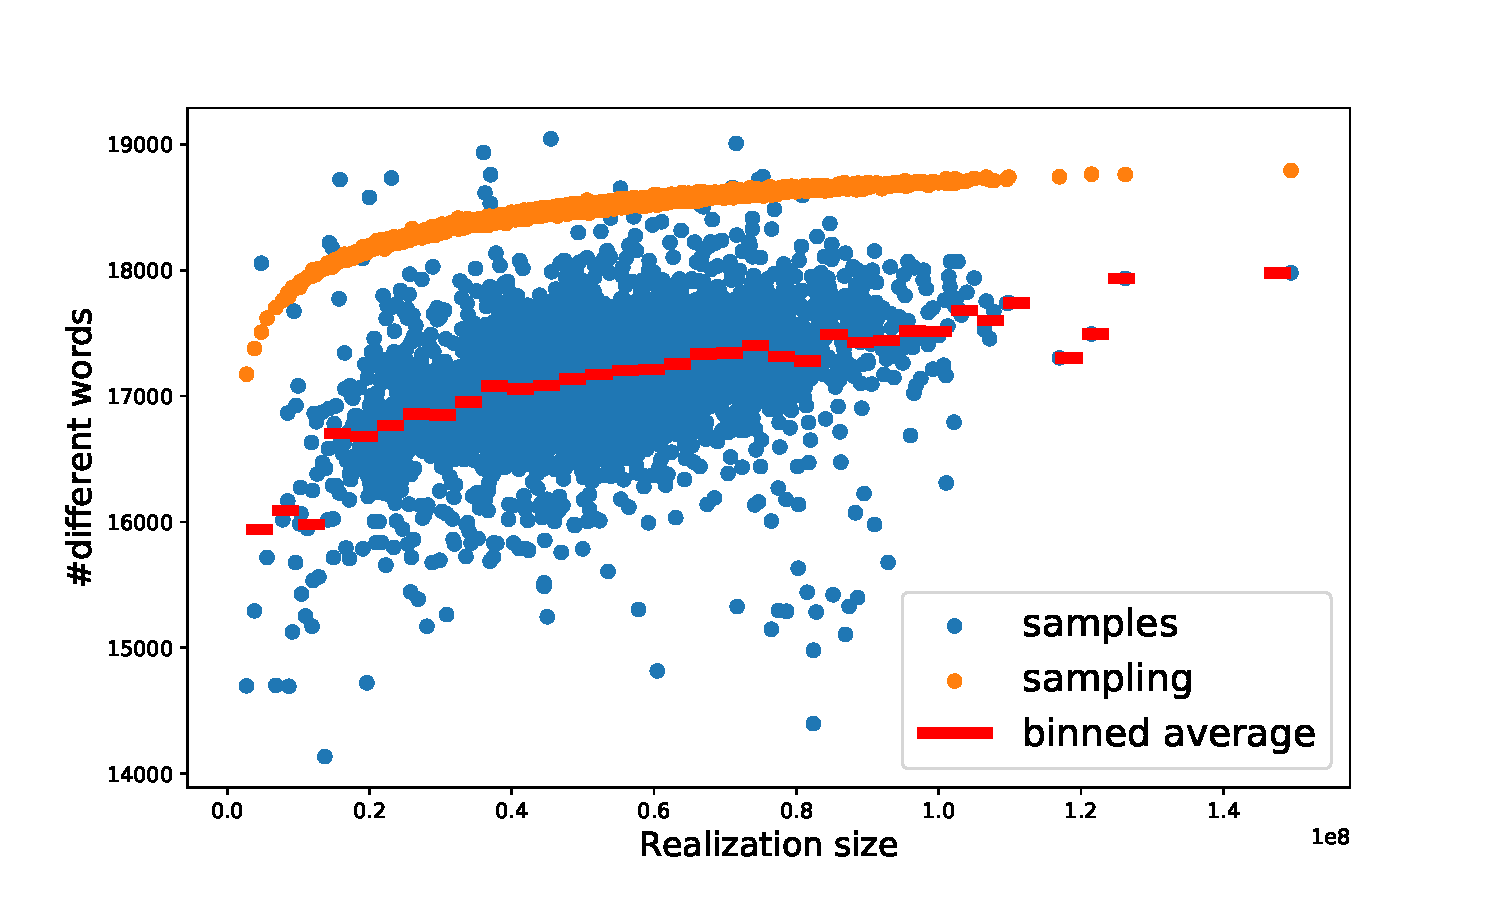
\includegraphics[width=0.95\linewidth]{pictures/structure/tcga/heaps_null.pdf}
    \end{minipage}
\hspace{2mm}
\begin{minipage}{0.5\textwidth}
    \centering
    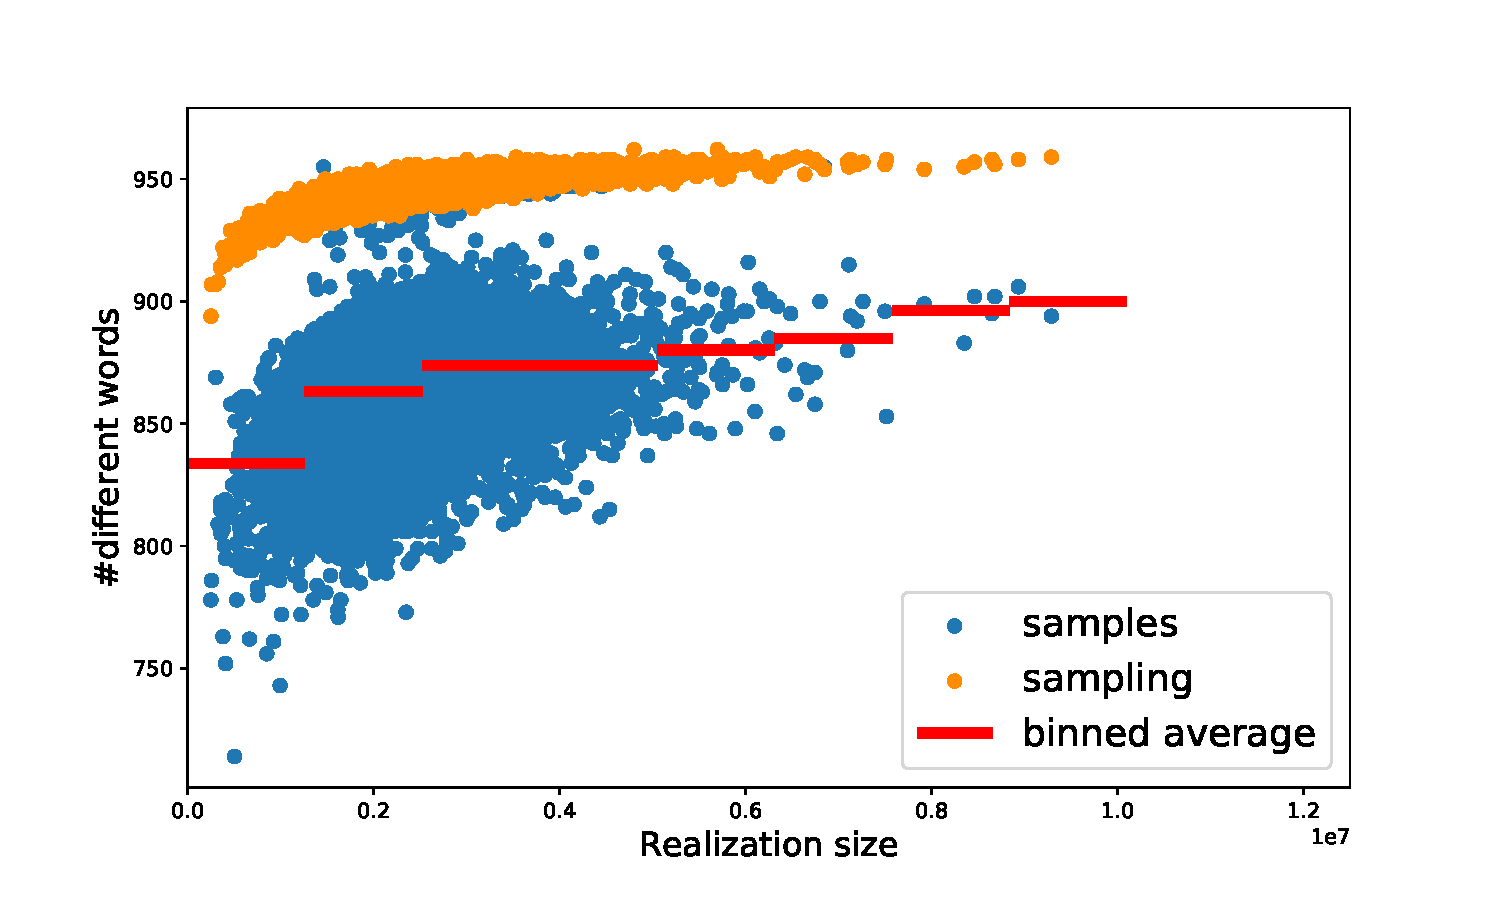
\includegraphics[width=0.95\linewidth]{pictures/structure/gtex/heaps_null.pdf}
    \end{minipage}
\caption{Heaps' law; TCGA(left) and GTEx (right). Sampling is reported for comparison.}
\label{fig:structure/heaps_null}
\end{figure}
Another way to see this is by looking at the histograms of the number of different genes expressed, actually the distribution of the~\ref{fig:structure/heaps_null} y-axis. Figure~\ref{fig:structure/diffwordsDistr_null} shows that these distributions are completely different if one looks at the data and the samples.
\begin{figure}[htb!]
\begin{minipage}{0.5\textwidth}
    \centering
    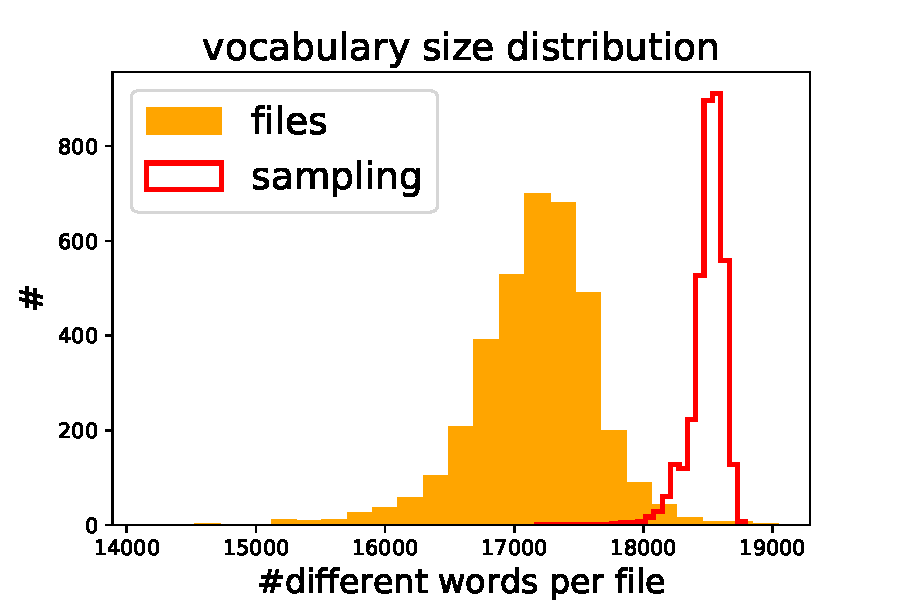
\includegraphics[width=0.95\linewidth]{pictures/structure/tcga/diffwordsDistr_null.pdf}
    \end{minipage}
\hspace{2mm}
\begin{minipage}{0.5\textwidth}
    \centering
    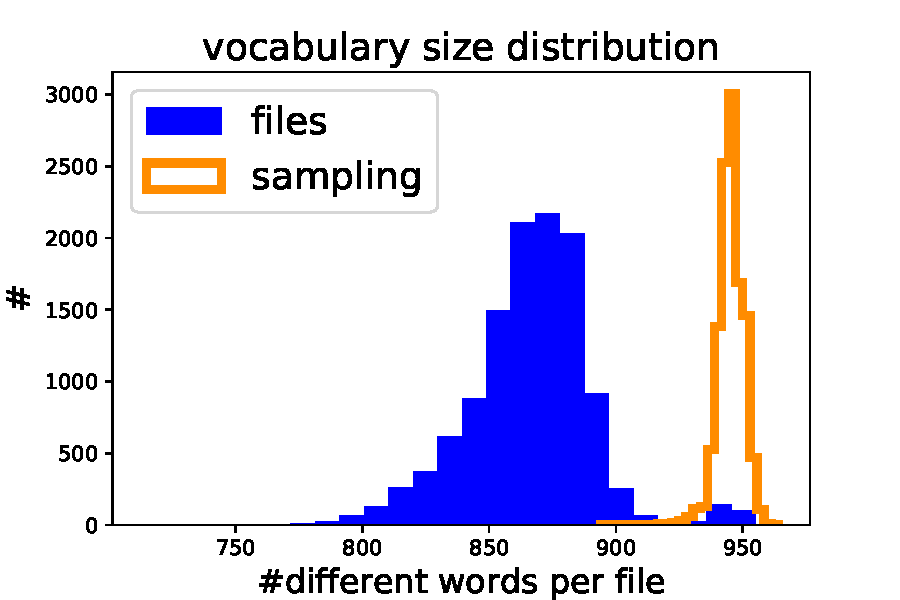
\includegraphics[width=0.95\linewidth]{pictures/structure/gtex/diffwordsDistr_null.pdf}
    \end{minipage}
\caption{Number of genes expressed in a sample; TCGA(left) and GTEx (right). The difference between the original data and sampling is evident.}
\label{fig:structure/diffwordsDistr_null}
\end{figure}

%%tissue differentation
%%tissue separation
\section{Statistical laws differentiate by tissue}
Observing the GTEx dataset of healthy samples it is possible to study how it is possible to see the tissue differentiation and how to study tissues' differences,~\cite{mele2014} suggests some approaches.

First of all, it could be interesting to study which is the fraction of transcriptome that can be explained by a certain number of genes.
To do this it is necessary to get all the samples of a given tissue. Then one estimates the average expression per each component (gene). At this point, one has the average abundance of each gene in a tissue, dividing by the sum of all the components it is possible to obtain the fraction of the total counts in the tissue due to each gene. Sorting from greater to smaller and integrating (cumulative summing) one have the fraction of transcript due to $1, 2, 3\dots$ genes. This is reported in figure~\ref{fig:structure/gtex/fraction_of_trascriptome}. This analysis is done using TPM to avoid biases due to gene lengths or to samples sizes.
\begin{figure}[htb!]
  \centering
  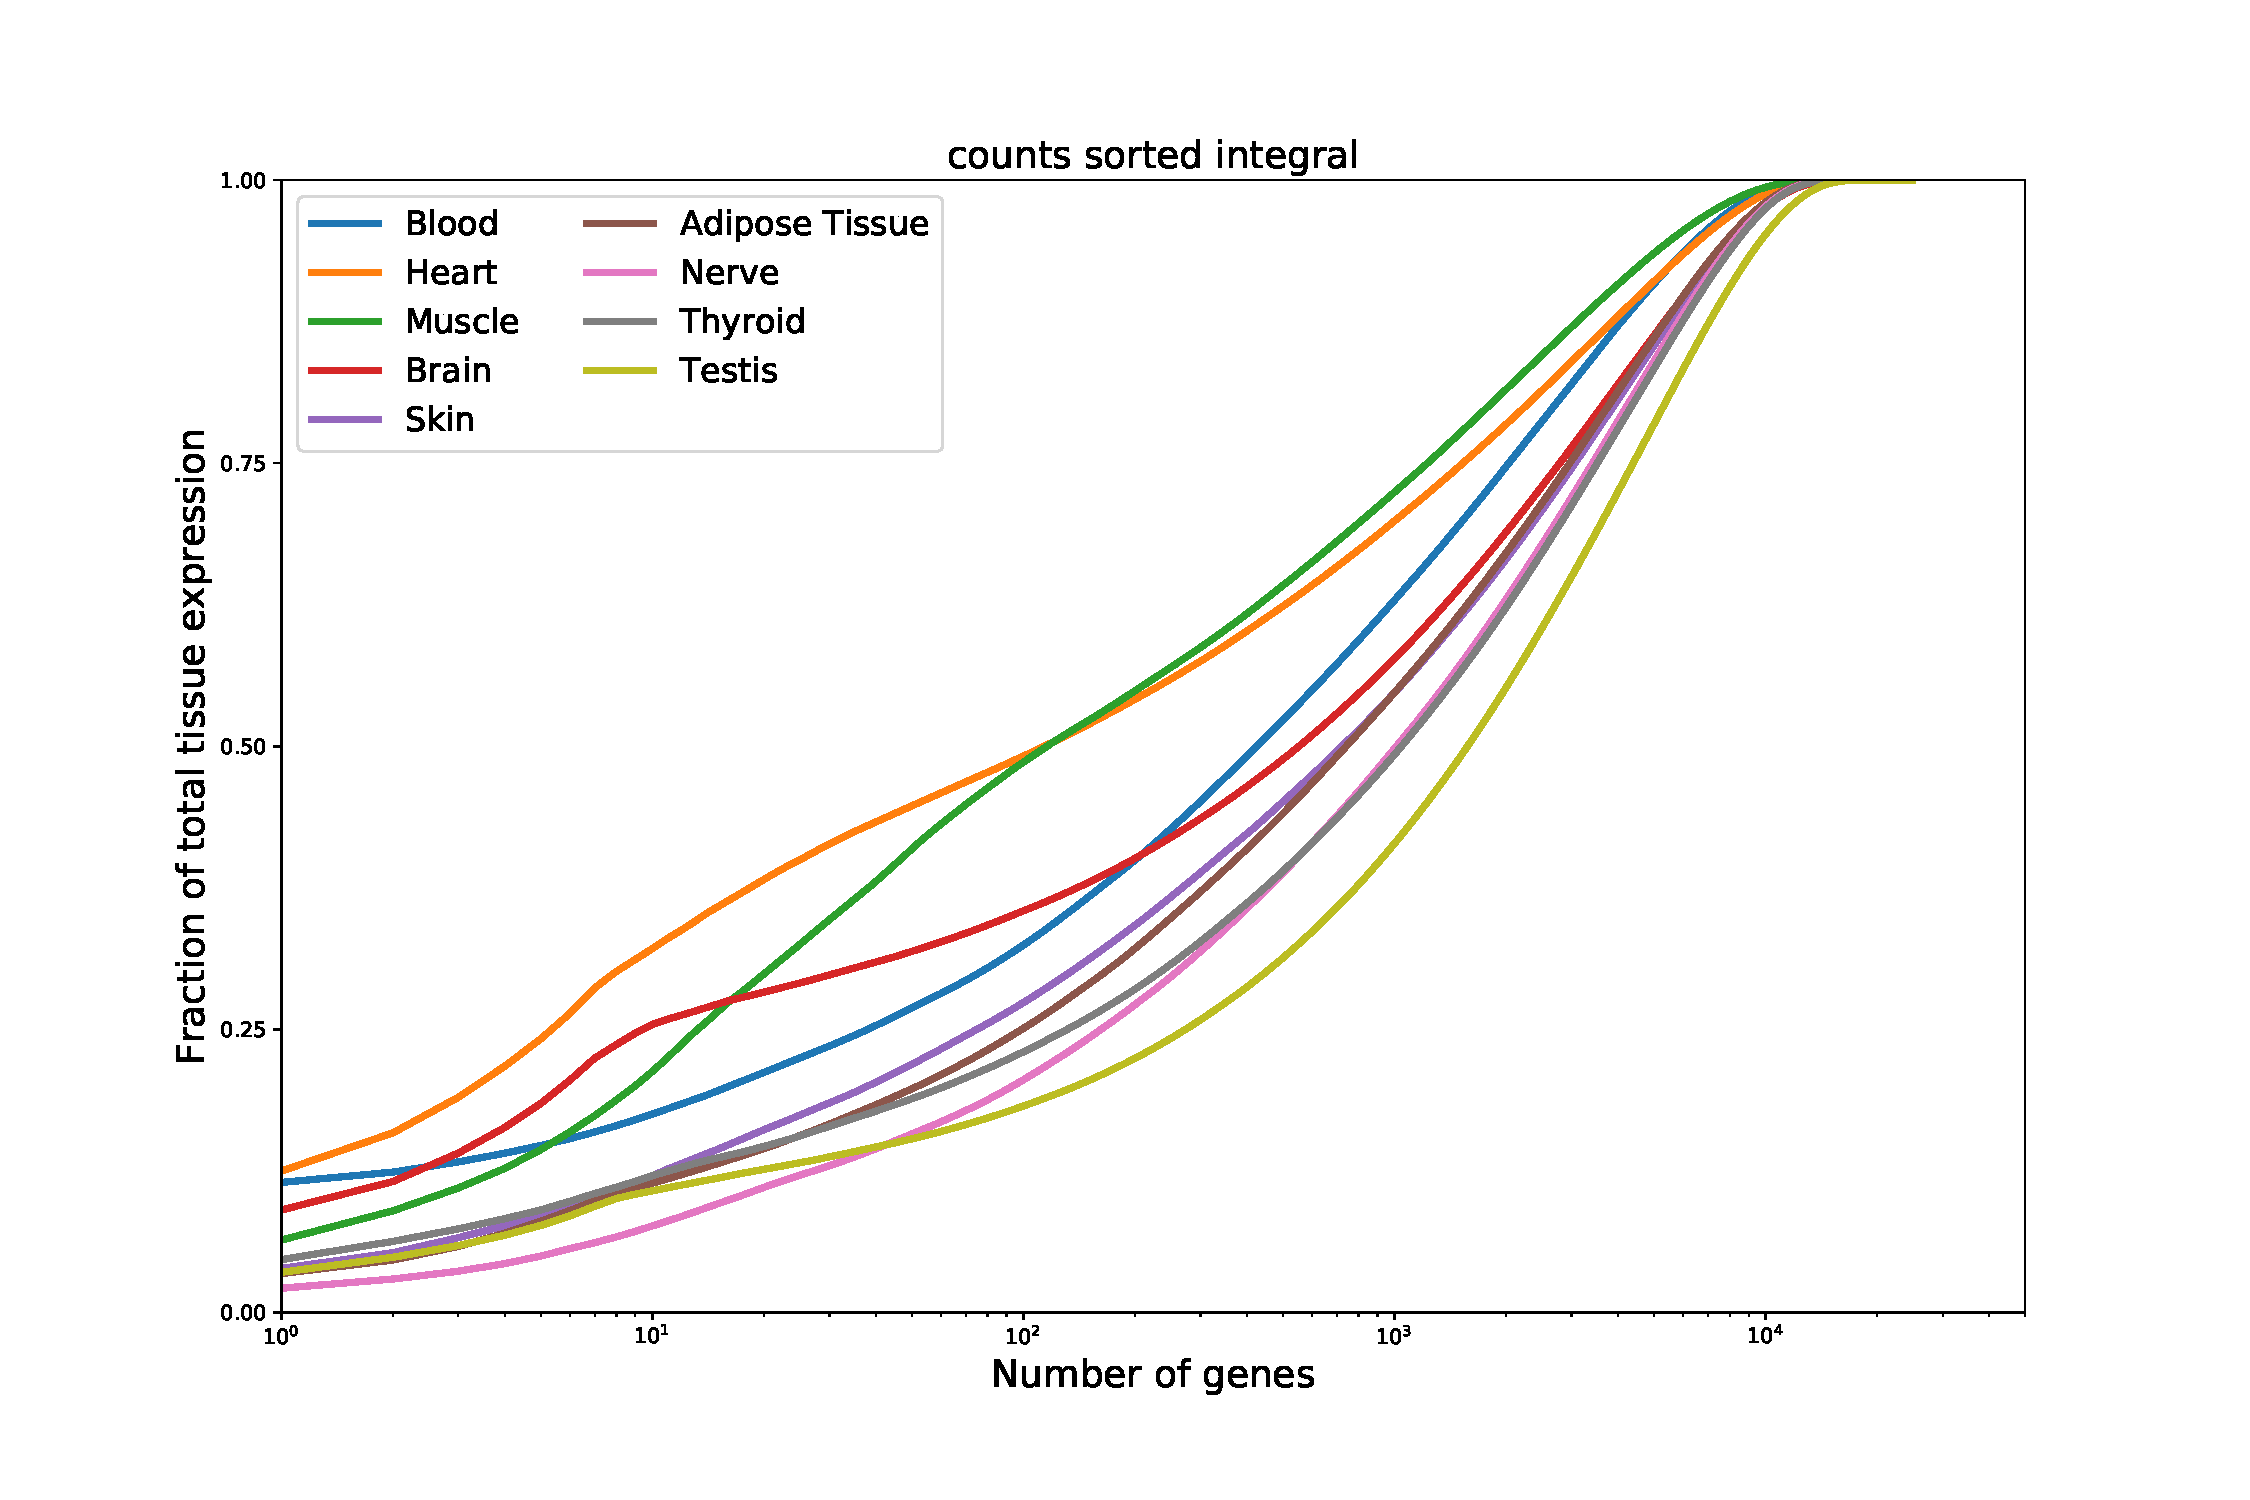
\includegraphics[width=0.7\linewidth]{pictures/structure/gtex/fraction_of_trascriptome.pdf}
  \caption{The integral of the sorted abundances for each tissue.}
  \label{fig:structure/gtex/fraction_of_trascriptome}
\end{figure}
Here, when a curve is steep it means that a few genes' expression represents a great fraction of the total size of the transcriptome. If a curve is smooth it means that many genes are necessary to describe the whole transcriptome for that particular tissue. This analysis shows that different tissues have a different complexity in terms of the number of genes necessary to build the transcriptome (in average). In figure~\ref{fig:structure/gtex/fraction_of_trascriptome_Brain} the same analysis is done for the sub-tissues of Brain, also this sub-type present a great separation.
\begin{figure}[htb!]
  \centering
  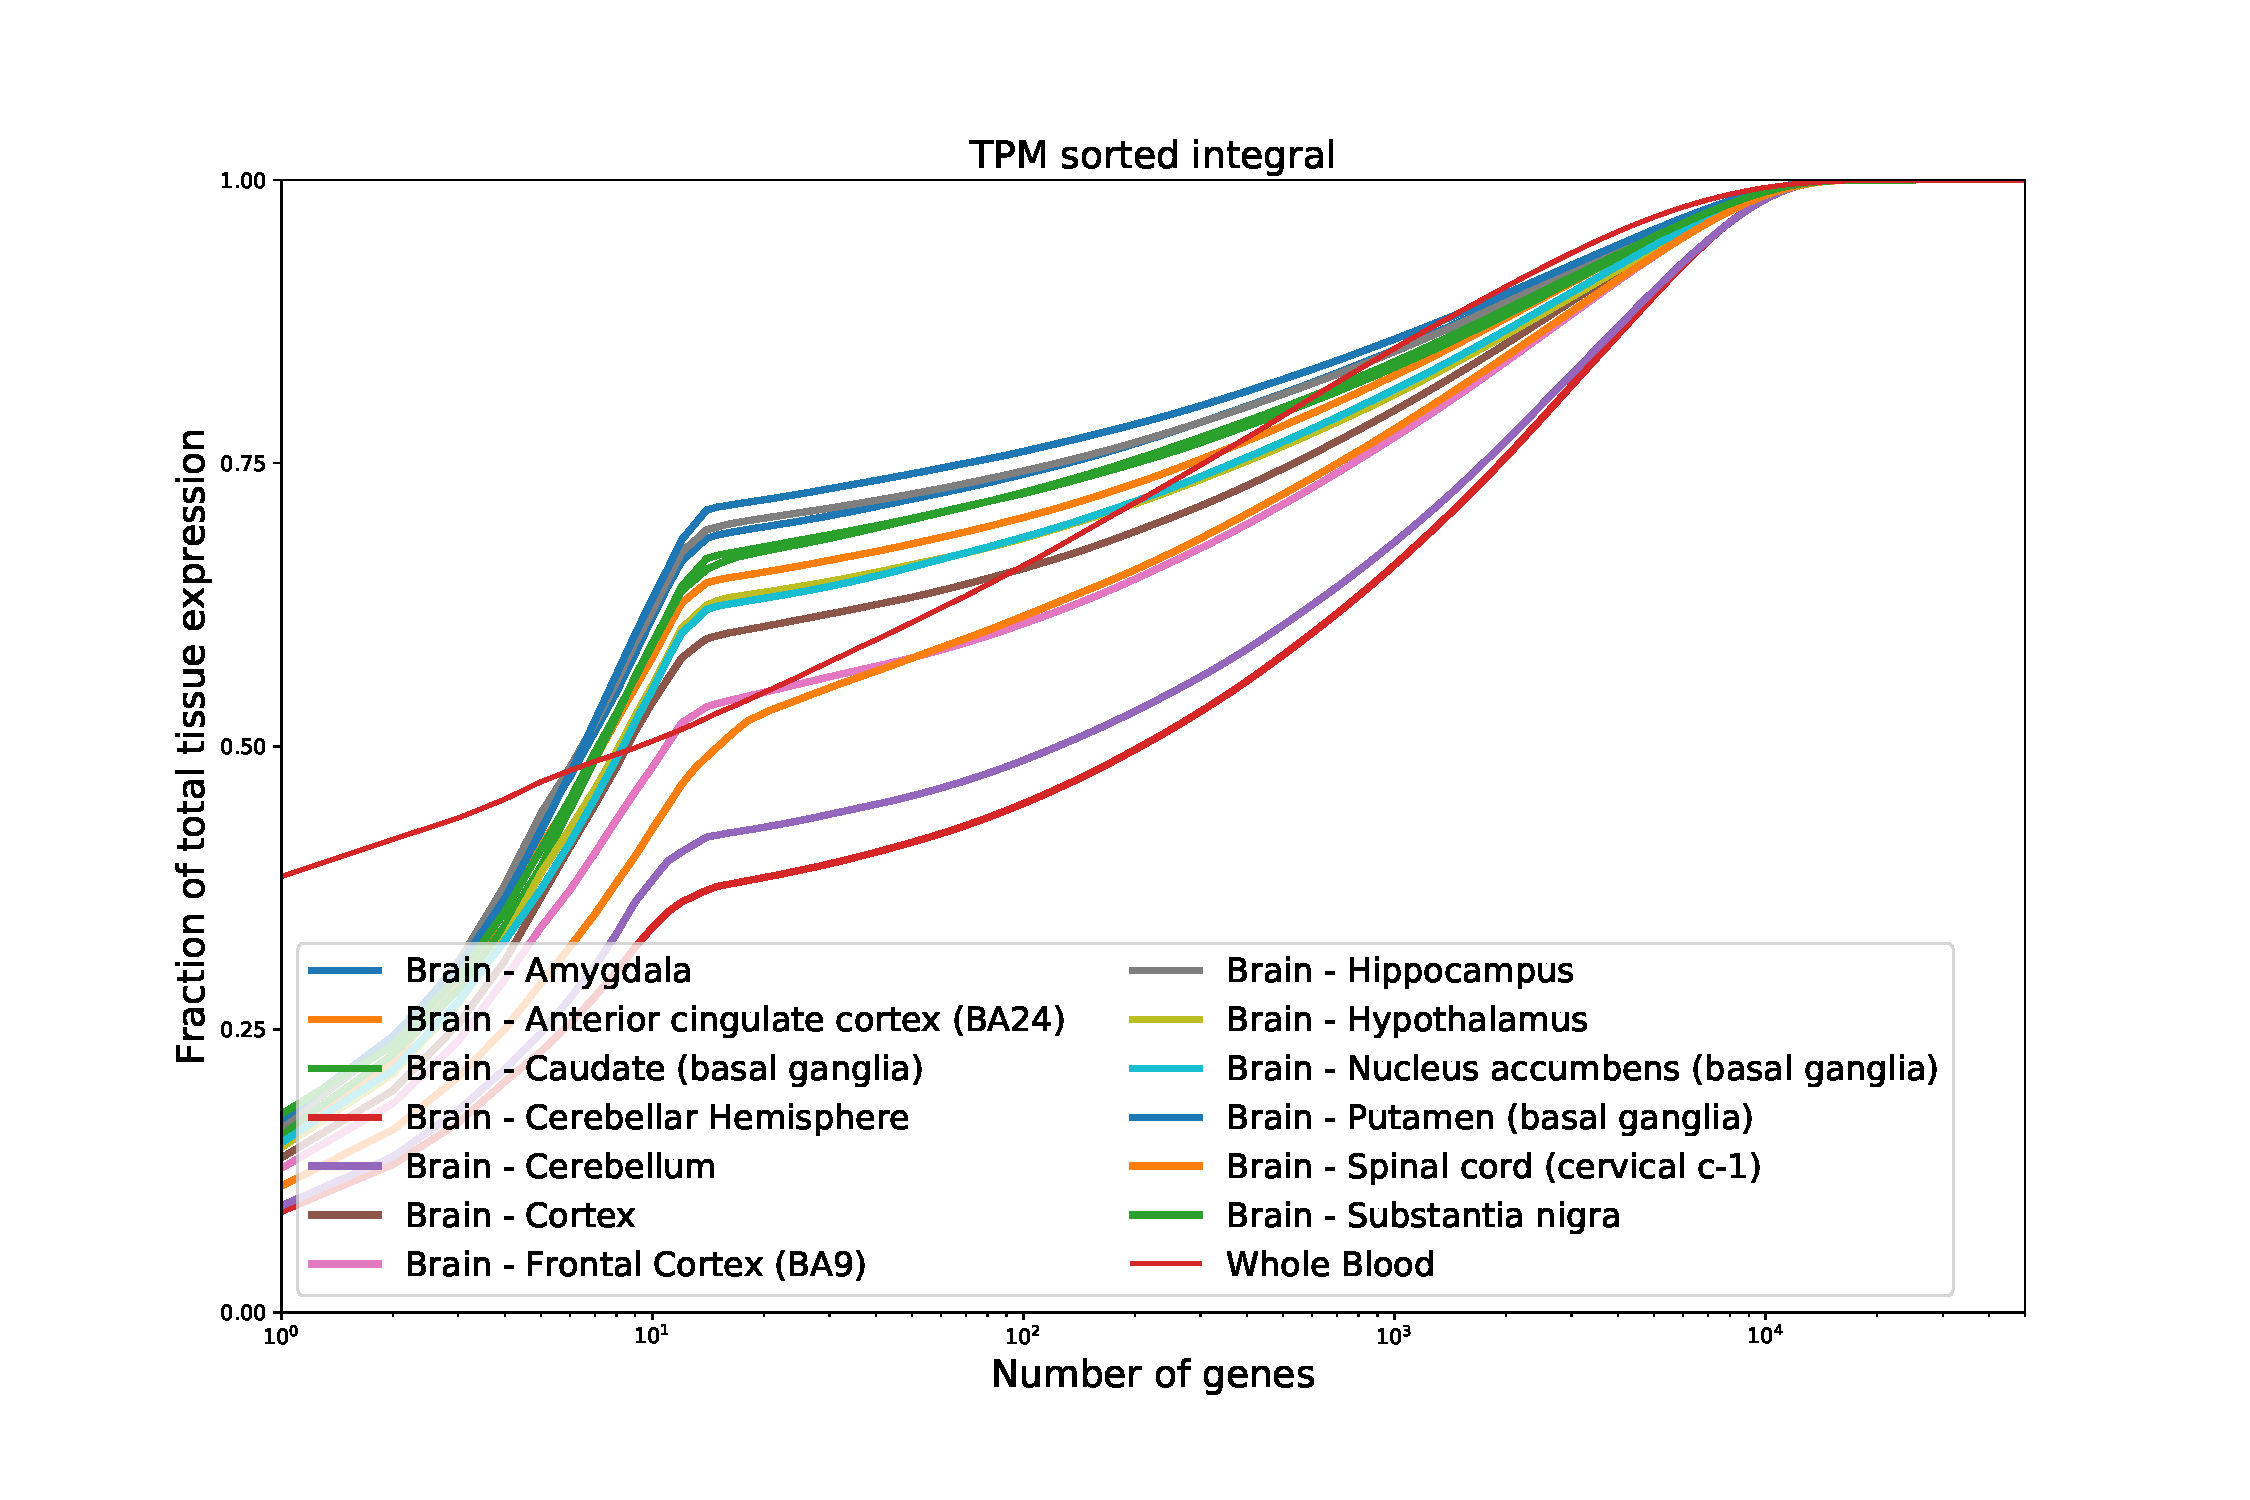
\includegraphics[width=0.65\linewidth]{pictures/structure/gtex/fraction_of_trascriptome_Brain.pdf}
  \caption{The integral of the sorted abundances for sub-types of Brain. This is done using TPM to avoid biases due to gene lengths. Blood is plotted for reference.}
  \label{fig:structure/gtex/fraction_of_trascriptome_Brain}
\end{figure}

Another way to interpret this analysis is thinking~\ref{fig:structure/gtex/fraction_of_trascriptome} as the integral of the Zipf's law. So it could be interesting to examine the Zipf one tissue a time. In figure~\ref{fig:structure/gtex/zipf_tissue} are reported the Zipf's law for some tissues with an extremal behaviour.
\begin{figure}[htb!]
  \centering
  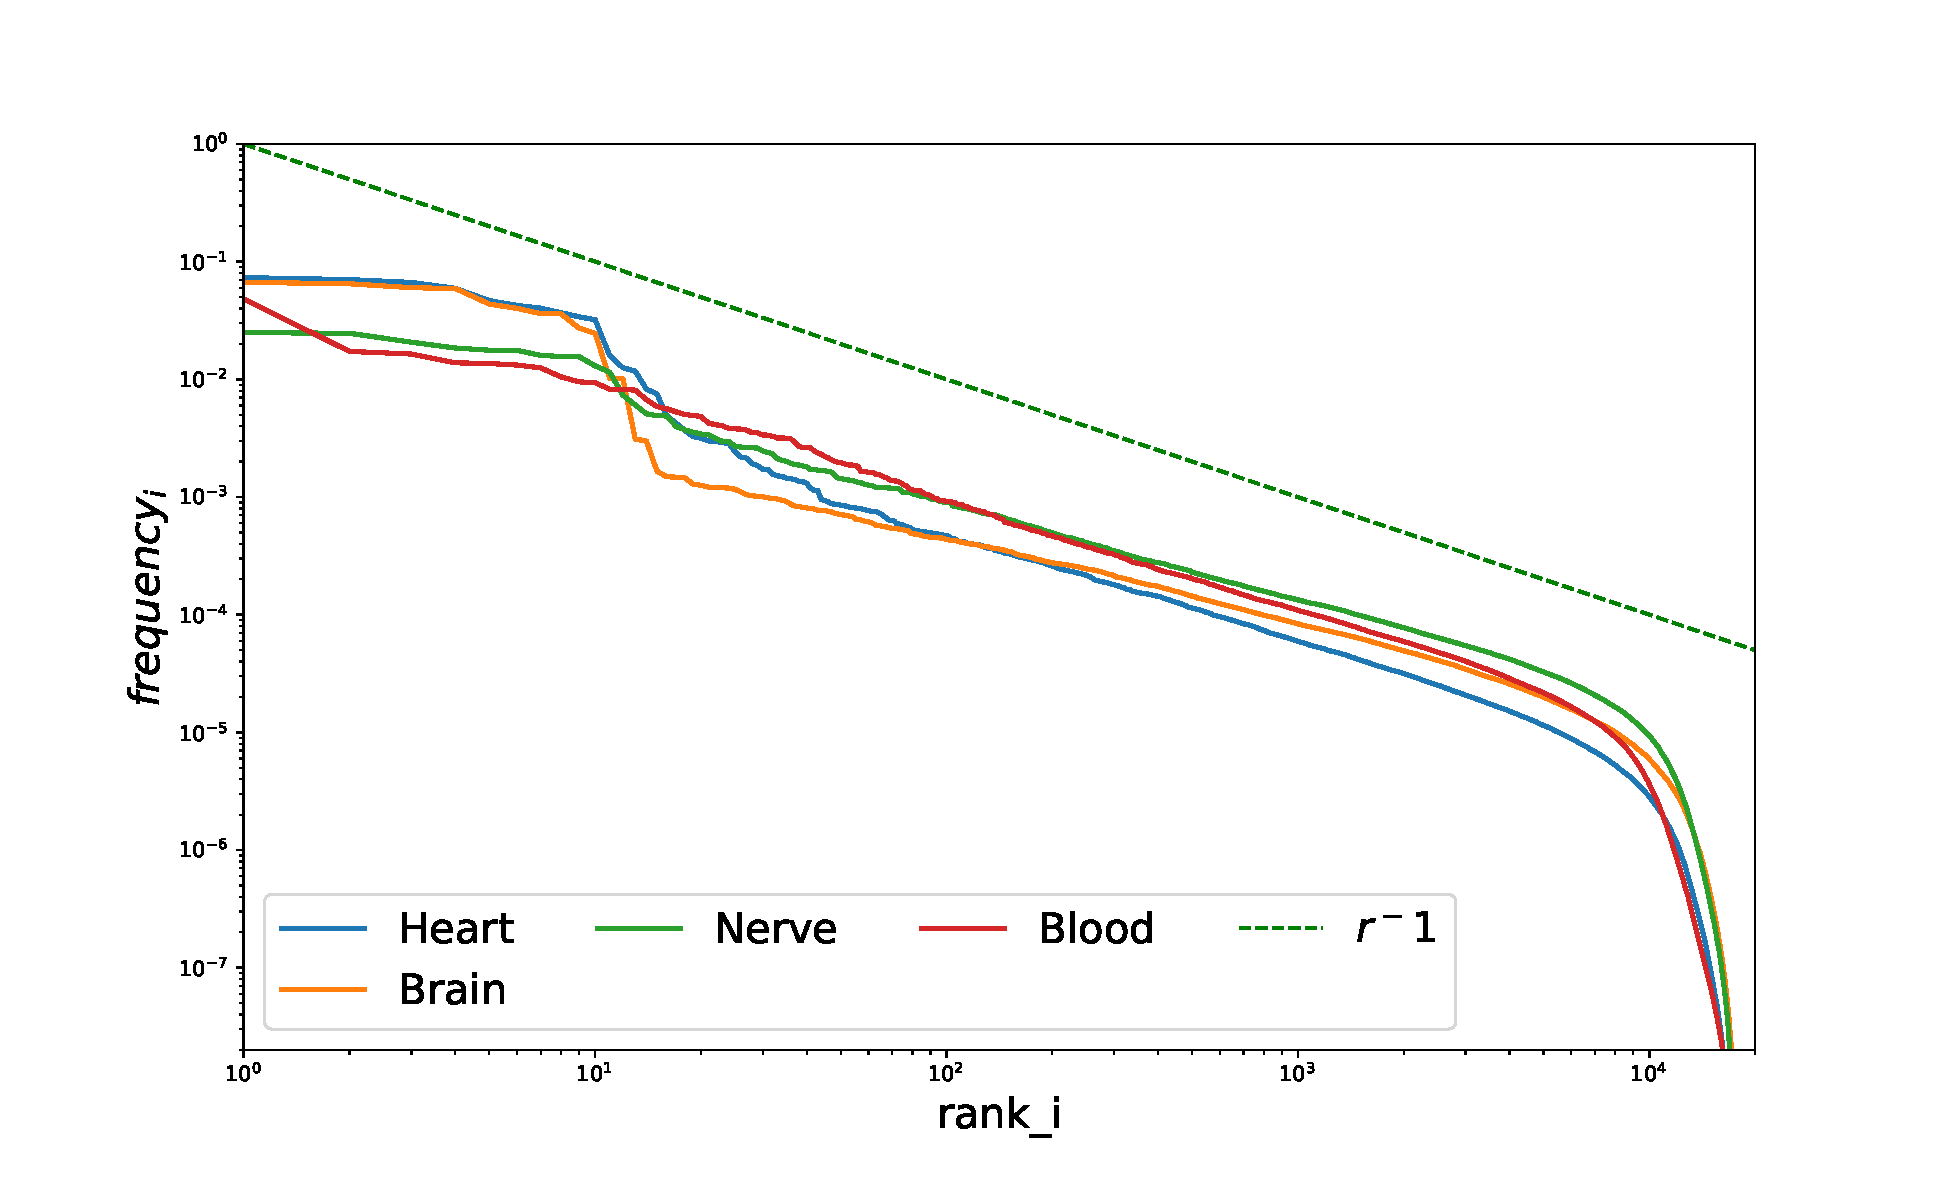
\includegraphics[width=0.45\linewidth]{pictures/structure/gtex/zipf_tissue.pdf}
  \caption{The integral of the sorted abundances for each tissue.}
  \label{fig:structure/gtex/zipf_tissue}
\end{figure}
From this point of view, each tissue has its particular slope. The steeper the Zipf the simplest is the tissue: the transcript can be described with few genes.

Coming back to the transcriptome analysis. In figure~\ref{fig:structure/gtex/fraction_of_trascriptome} the point where the curve reaches $1$ corresponds to the total number of genes expressed, the remaining ones have a $0$ expression and do not contribute to the transcript. This can be visualized again with the Heaps' law: the number of genes expressed seen in the Heaps' law plot is the number of genes necessary to explain the whole transcriptome. In figure~\ref{fig:structure/gtex/heaps_tissue}, it is evident that there is some kind of tissue differentiation even when looking at the Heaps' law. In other words, two samples with the same size but of different tissues have a different number of genes expressed.
\begin{figure}[htb!]
  \centering
  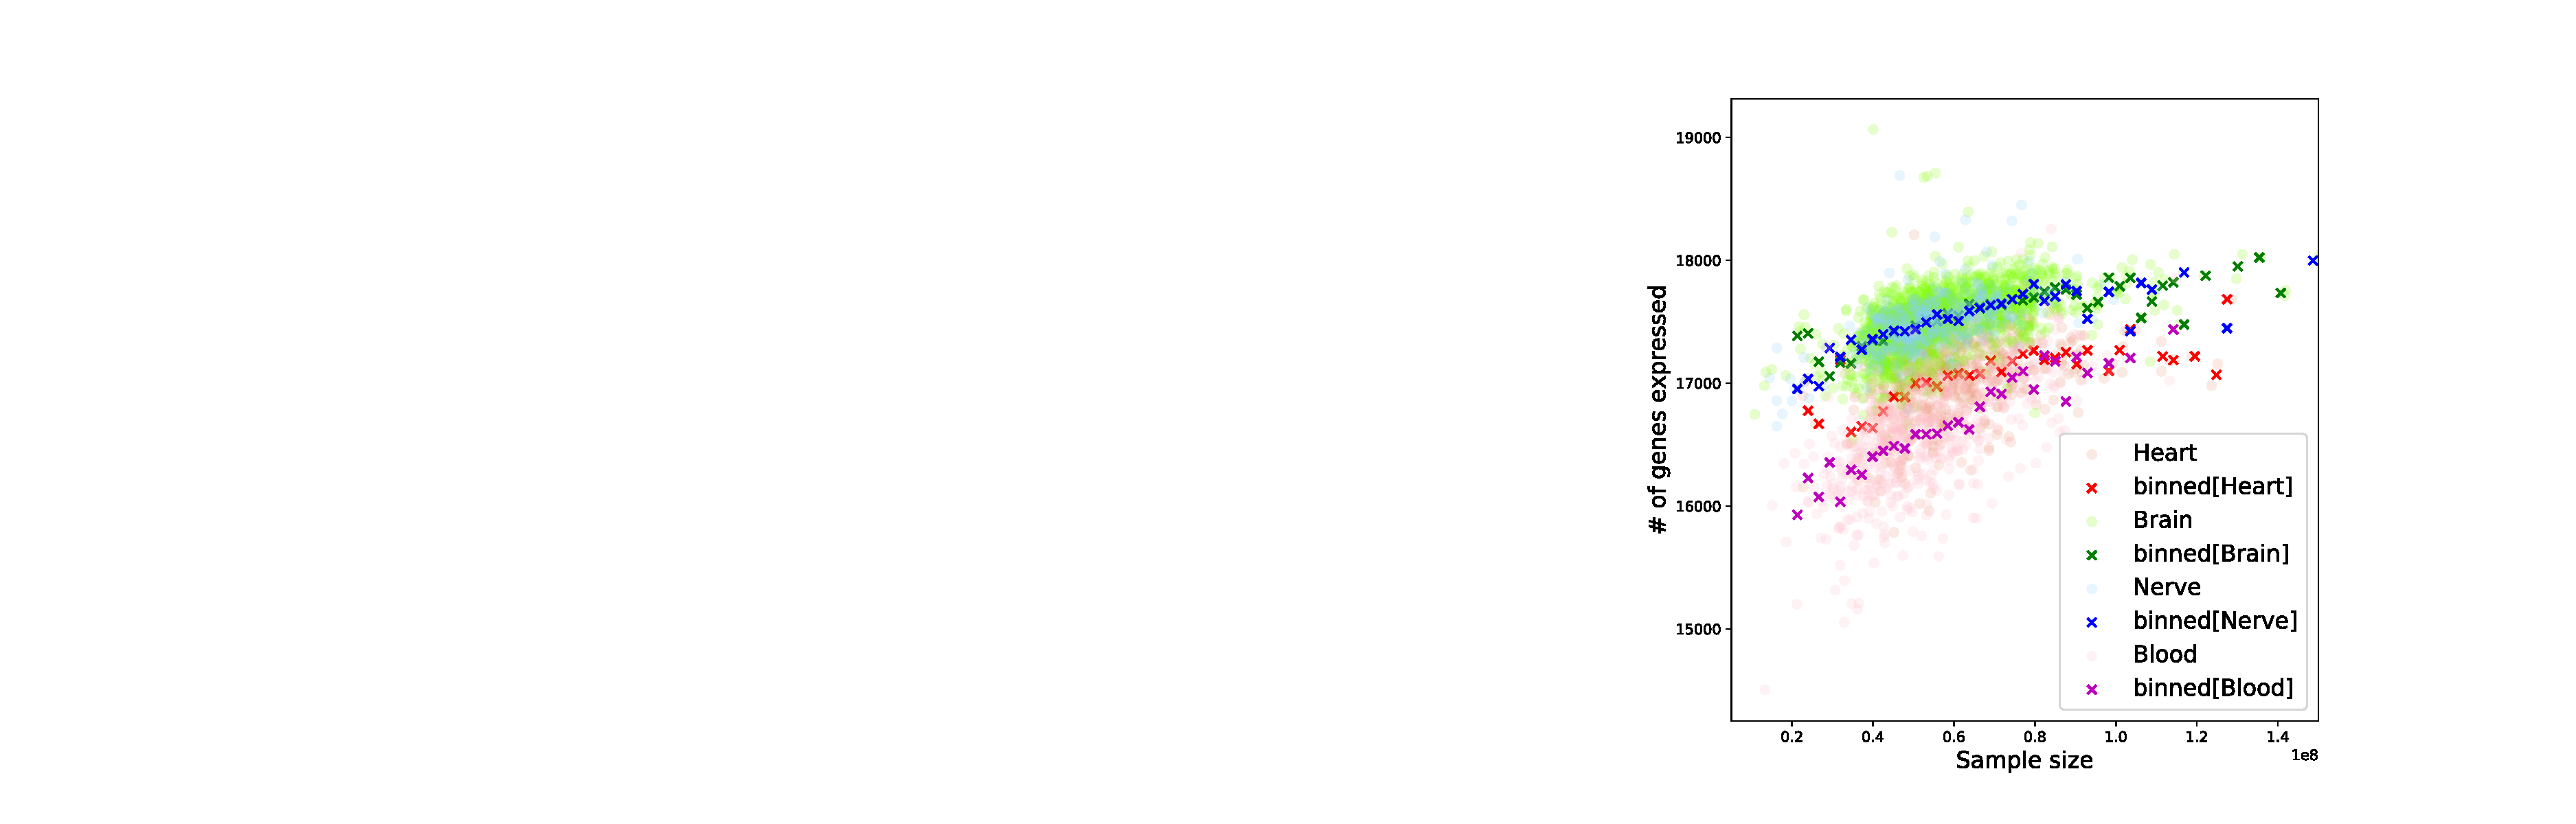
\includegraphics[width=0.5\linewidth]{pictures/structure/gtex/heaps_tissue.pdf}
  \caption{The integral of the sorted abundances for each tissue. This plot was done using counts, using TPM it is not possible because the size on the x-axis is a would be a constant.}
  \label{fig:structure/gtex/heaps_tissue}
\end{figure}
The same analysis can be made by looking at the disease type of cancer samples. In this case, there is no evident differentiation as shown in figure~\ref{fig:structure/tcga/fraction_of_trascriptome_disease}. The only diseases that behave differently are \textit{Parangliomas}, but these are associated only to Brain, so the differentiation seen is just a Brain separation. This means that separate diseases would be tricky and much more difficult than just separate tissues.
\begin{figure}[htb!]
  \centering
  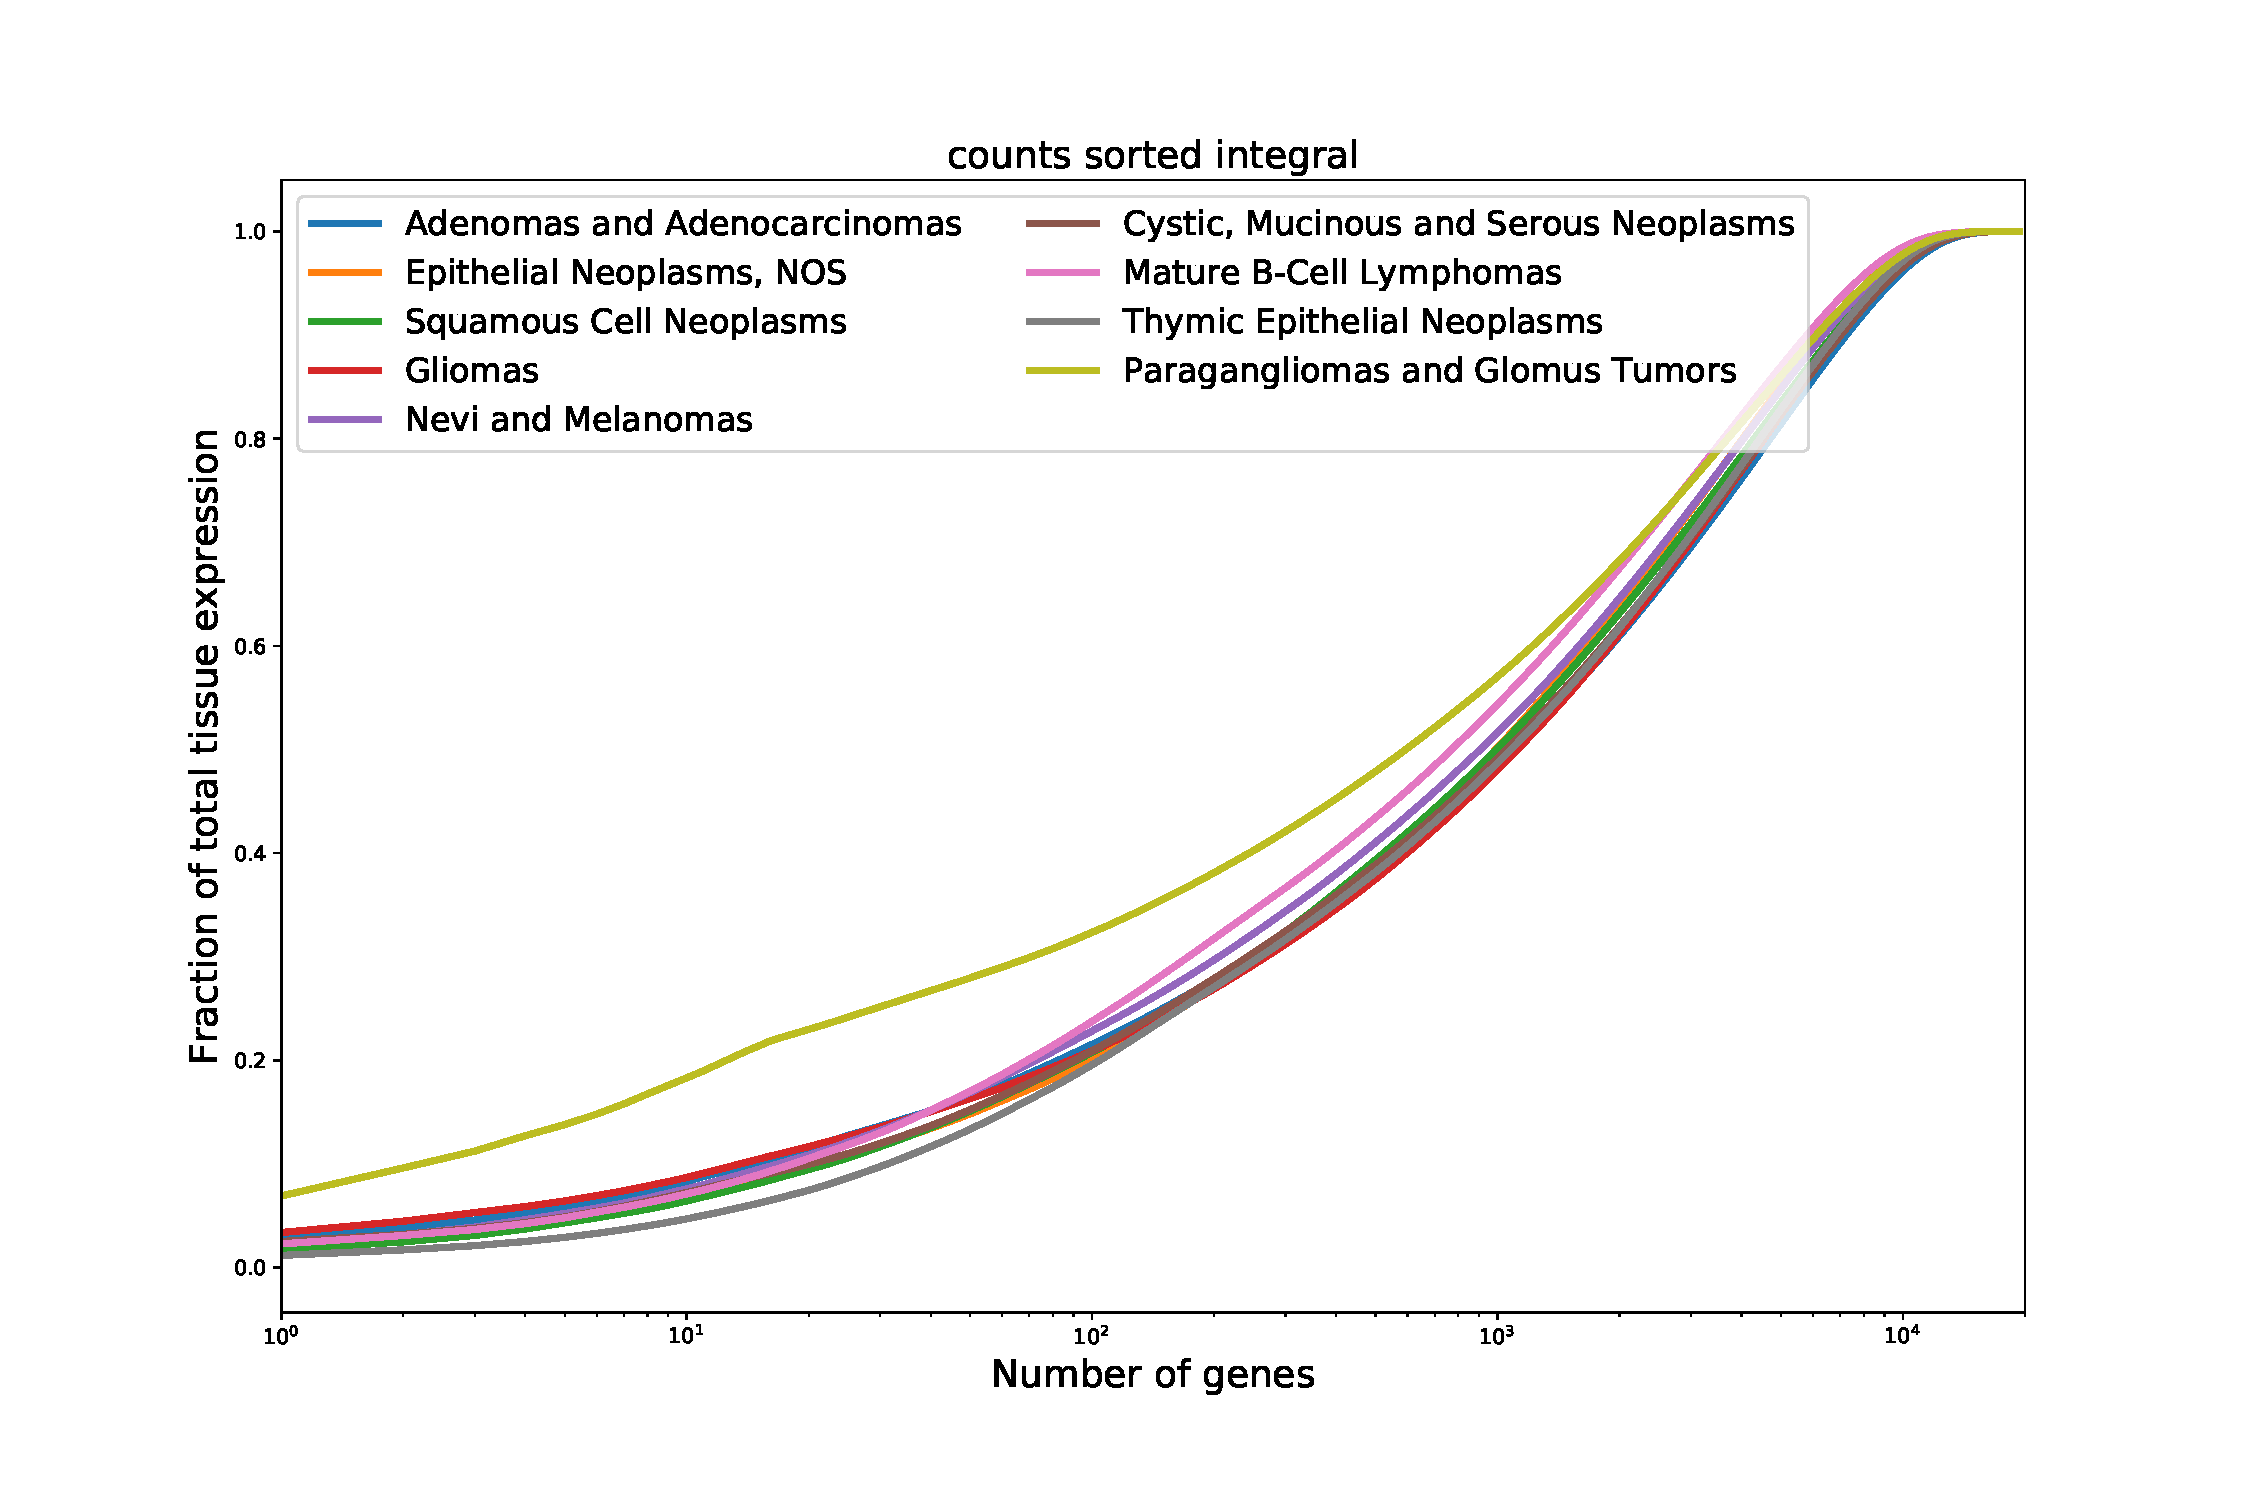
\includegraphics[width=0.8\linewidth]{pictures/structure/tcga/fraction_of_trascriptome_disease.pdf}
  \caption{The integral of the sorted abundances for each disease type.}
  \label{fig:structure/tcga/fraction_of_trascriptome_disease}
\end{figure}

\FloatBarrier
All these analyses suggest that there must be a sort of hidden structure in the data that is somehow related to the tissue each sample comes from. In particular, there are many Zipf's laws hidden behind the data and each sample is build looking at one of these a time. Also given two samples with a similar size, it happens that the number of genes necessary to build that realization is not always the same (shown by Heaps' law) and it is somehow related to the tissue of the sample.

In conclusion, some interesting laws were found that some statistical.

...